\chapter{Klank}\fancyfoot[LO,RE]{Fisika: Golwe, Klank en Lig}

    \setcounter{figure}{1}
    \setcounter{subfigure}{1}
    \label{9b5d72dd5f0585e544578ab90a9956a8}
         \section{Inleiding}
    \nopagebreak
    \label{m38799*cid2}
\label{m38799*id183123}Het jy al ooit gedink hoe wonderlik die sintuig van gehoor is? Dis merkwaardig dat ons so 'n wye spektrum van klank kan hoor en kan bepaal uit watter rigting die klank vandaan kom. Hoe word klanke gevorm dat ons kan hoor? Enige iets wat 'n versteuring in die lug veroorsaak, skep 'n puls wat weg beweeg van die punt van oorsprong. As die puls 'n mens se oor binnegaan veroorsaak dit 'n vibrasie in die oordrom, en dit is hoe 'n mens hoor. As die oorsrpong van die puls 'n reeks van pulse is dan word die versteuring 'n golf genoem. \par
\chapterstartvideo{VPdxu}

In die algemeen word aanvaar dat klank 'n golf is. Klankgolwe is longitudinale drukgolwe wat beteken die golf bestaan uit verdigtings en verdunnings van lugdruk.

\subsection*{Klankgolwe}
            \nopagebreak
 'n Stemvurk is 'n instrument wat deur musikante gebruik work om 'n klankgolf met 'n spesifieke frekwensie op te wek. Dit word dikwels gebruik om musiekinstrumente te stem.

\begin{minipage}{.5\textwidth}
Klankgolwe wat van die stemvurk afkomstig is word veroorsaak deur vibrasies van die stemvurk wat met omliggende lugmolekules in wisselwerkingtree. Soos die lugmolekules saamgepers word, vorm 'n verdigting. Die deeltjies agter die verdigting beweeg verder van mekaar om 'n verdunning to vorm. Soos die deeltjies aanhou om teen mekaar te druk, beweeg die klankgolf deur lug. Di\'{e} beweging van deeltjies veroorsaak 'n konstante verandering in druk. Daarom is klankgolwe, drukgolwe. Dit beteken dat klankgolwe vinniger sal beweeg in 'n medium waar die deeltjies nader aanmekaar is.\par

\mindsetvid{Science of sound}{VPdya}
\end{minipage}
\begin{minipage}{.5\textwidth}\begin{center}
\textbf{Stemvurk}\par
    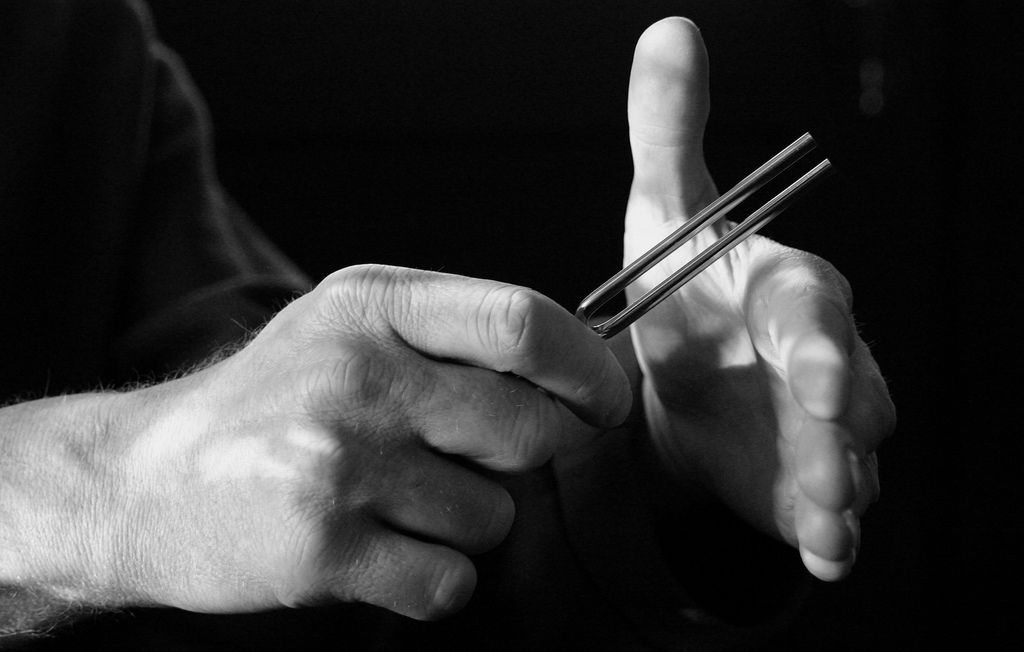
\includegraphics[width=0.8\textwidth]{../Grade10/photos/TuningFork2_Flickr_amonya.jpg}\par
\textit{Foto deur amonya op Flickr}
\end{center}
\end{minipage}

Klankgolwe beweeg vinniger in vloeistowwe soos water as deur lug, want water is digter as lug (die deeltjies is nader aanmekaar). Klankgolwe beweeg nog vinniger in vaste stowwe as in vloeistowwe.
    \setcounter{subfigure}{0}
	\begin{figure}[H] % horizontal\label{m38783*uid18}
    \begin{center}
\scalebox{1} % Change this value to rescale the drawing.
{
\begin{pspicture}(0,-1.3159375)(10.862187,1.3159375)
\psline[linewidth=0.04cm](1.5942917,-0.29788056)(1.8169739,-0.30129474)
\psline[linewidth=0.04cm](1.8169739,-0.30129474)(1.8345535,0.44497925)
\psline[linewidth=0.04cm](1.9030713,0.44392854)(1.8835384,-0.3852649)
\psline[linewidth=0.04cm](1.8835384,-0.3852649)(1.7636325,-0.38342634)
\psline[linewidth=0.04cm](1.5771624,-0.29761782)(1.5947421,0.44865623)
\psline[linewidth=0.04cm](1.5262243,0.4497069)(1.5066916,-0.3794867)
\psline[linewidth=0.04cm](1.6437267,-0.38158786)(1.5238208,-0.37974924)
\psline[linewidth=0.04cm](1.6269228,-0.36750528)(1.6171566,-0.7821023)
\psline[linewidth=0.04cm](1.6171566,-0.7821023)(1.7541916,-0.7842031)
\psline[linewidth=0.04cm](1.7541916,-0.7842031)(1.7636325,-0.38342634)
\psline[linewidth=0.04cm](1.8345535,0.44497925)(1.9030713,0.44392854)
\psline[linewidth=0.04cm](1.5947421,0.44865623)(1.5262243,0.4497069)
\psdots[dotsize=0.04](2.0484376,0.2296875)
\psdots[dotsize=0.04](2.1284375,0.2496875)
\psdots[dotsize=0.04](2.0884376,0.2096875)
\psdots[dotsize=0.04](2.0084374,0.1296875)
\psdots[dotsize=0.04](2.1084375,0.0896875)
\psdots[dotsize=0.04](2.1684375,0.1696875)
\psdots[dotsize=0.04](2.1284375,0.1696875)
\psdots[dotsize=0.04](2.0684376,0.1296875)
\psdots[dotsize=0.04](2.0684376,-0.0103125)
\psdots[dotsize=0.04](2.1484375,-0.0303125)
\psdots[dotsize=0.04](2.1684375,0.1296875)
\psdots[dotsize=0.04](2.2684374,0.1896875)
\psdots[dotsize=0.04](2.2884376,0.1096875)
\psdots[dotsize=0.04](2.2884376,0.0096875)
\psdots[dotsize=0.04](2.2484374,-0.0103125)
\psdots[dotsize=0.04](2.1884375,-0.1103125)
\psdots[dotsize=0.04](2.0684376,-0.1503125)
\psdots[dotsize=0.04](1.9684376,-0.0903125)
\psdots[dotsize=0.04](2.0084374,-0.0103125)
\psdots[dotsize=0.04](2.1684375,-0.1103125)
\psdots[dotsize=0.04](2.2284374,-0.1503125)
\psdots[dotsize=0.04](2.2284374,0.0296875)
\psdots[dotsize=0.04](2.1884375,0.0896875)
\psdots[dotsize=0.04](2.2284374,0.2296875)
\psdots[dotsize=0.04](2.3084376,0.1696875)
\psdots[dotsize=0.04](2.3084376,-0.0703125)
\psdots[dotsize=0.04](2.2684374,-0.1303125)
\psdots[dotsize=0.04](2.1884375,-0.2103125)
\psdots[dotsize=0.04](2.1084375,-0.2103125)
\psdots[dotsize=0.04](2.0484376,-0.1703125)
\psdots[dotsize=0.04](1.9884375,-0.1903125)
\psdots[dotsize=0.04](2.0084374,-0.2103125)
\psdots[dotsize=0.04](2.0884376,-0.2303125)
\psdots[dotsize=0.04](2.1884375,-0.2903125)
\psdots[dotsize=0.04](2.2684374,-0.2303125)
\psdots[dotsize=0.04](2.3084376,-0.1303125)
\psdots[dotsize=0.04](2.3084376,0.0096875)
\psdots[dotsize=0.04](2.0484376,0.0496875)
\psdots[dotsize=0.04](2.0884376,-0.0903125)
\psdots[dotsize=0.04](2.0284376,-0.0703125)
\psdots[dotsize=0.04](2.2284374,0.1296875)
\psdots[dotsize=0.04](2.0084374,-0.2703125)
\psdots[dotsize=0.04](2.2684374,0.2496875)
\psdots[dotsize=0.04](2.3484375,0.2496875)
\psdots[dotsize=0.04](2.3484375,0.1696875)
\psdots[dotsize=0.04](2.4284375,0.2296875)
\psdots[dotsize=0.04](2.4084375,0.2296875)
\psdots[dotsize=0.04](2.4484375,0.0496875)
\psdots[dotsize=0.04](2.4284375,0.1496875)
\psdots[dotsize=0.04](2.3484375,0.1096875)
\psdots[dotsize=0.04](2.3684375,0.0096875)
\psdots[dotsize=0.04](2.3684375,0.0096875)
\psdots[dotsize=0.04](2.3084376,0.0496875)
\psdots[dotsize=0.04](2.4484375,-0.0903125)
\psdots[dotsize=0.04](2.3684375,-0.1303125)
\psdots[dotsize=0.04](2.3284376,-0.1103125)
\psdots[dotsize=0.04](2.4084375,-0.0703125)
\psdots[dotsize=0.04](2.4684374,-0.0303125)
\psdots[dotsize=0.04](2.4684374,-0.1503125)
\psdots[dotsize=0.04](2.4284375,-0.1903125)
\psdots[dotsize=0.04](2.3484375,-0.2303125)
\psdots[dotsize=0.04](2.3084376,-0.2503125)
\psdots[dotsize=0.04](2.3884375,-0.2903125)
\psdots[dotsize=0.04](2.4884374,-0.2503125)
\psdots[dotsize=0.04](2.2284374,-0.0503125)
\psdots[dotsize=0.04](2.1084375,-0.2903125)
\psdots[dotsize=0.04](2.0084374,0.0696875)
\psdots[dotsize=0.04](2.0084374,0.2296875)
\psdots[dotsize=0.04](2.0484376,0.2696875)
\psdots[dotsize=0.04](2.4484375,0.1496875)
\psdots[dotsize=0.04](2.4684374,0.2296875)
\psdots[dotsize=0.04](2.5484376,0.2296875)
\psdots[dotsize=0.04](2.7284374,0.1896875)
\psdots[dotsize=0.04](2.7684374,-0.0703125)
\psdots[dotsize=0.04](2.5884376,-0.0103125)
\psdots[dotsize=0.04](2.6684375,0.1096875)
\psdots[dotsize=0.04](2.8684375,0.0296875)
\psdots[dotsize=0.04](3.3084376,-0.0903125)
\psdots[dotsize=0.04](3.1484375,0.0896875)
\psdots[dotsize=0.04](2.9884374,0.1296875)
\psdots[dotsize=0.04](3.0084374,0.1896875)
\psdots[dotsize=0.04](3.2084374,0.1696875)
\psdots[dotsize=0.04](2.8084376,0.2696875)
\psdots[dotsize=0.04](3.0684376,-0.0703125)
\psdots[dotsize=0.04](2.6284375,-0.2303125)
\psdots[dotsize=0.04](2.7884376,-0.2703125)
\psdots[dotsize=0.04](3.0284376,-0.2503125)
\psdots[dotsize=0.04](2.9084375,-0.0903125)
\psdots[dotsize=0.04](3.2284374,-0.2503125)
\psdots[dotsize=0.04](3.2684374,0.0296875)
\psdots[dotsize=0.04](3.1284375,0.2496875)
\psdots[dotsize=0.04](3.3284376,0.2496875)
\psdots[dotsize=0.04](3.4884374,0.2096875)
\psdots[dotsize=0.04](3.6884375,0.2496875)
\psdots[dotsize=0.04](3.6484375,0.0696875)
\psdots[dotsize=0.04](3.6084375,-0.1103125)
\psdots[dotsize=0.04](3.3484375,0.0496875)
\psdots[dotsize=0.04](3.4884374,0.0696875)
\psdots[dotsize=0.04](3.4484375,-0.1703125)
\psdots[dotsize=0.04](3.3284376,-0.2303125)
\psdots[dotsize=0.04](3.5484376,-0.2703125)
\psdots[dotsize=0.04](3.6684375,-0.2703125)
\psdots[dotsize=0.04](3.7884376,0.2496875)
\psdots[dotsize=0.04](3.8684375,0.2696875)
\psdots[dotsize=0.04](3.8284376,0.2296875)
\psdots[dotsize=0.04](3.7484374,0.1496875)
\psdots[dotsize=0.04](3.8484375,0.1096875)
\psdots[dotsize=0.04](3.9084375,0.1896875)
\psdots[dotsize=0.04](3.8684375,0.1896875)
\psdots[dotsize=0.04](3.8084376,0.1496875)
\psdots[dotsize=0.04](3.8084376,0.0096875)
\psdots[dotsize=0.04](3.8884375,-0.0103125)
\psdots[dotsize=0.04](3.9084375,0.1496875)
\psdots[dotsize=0.04](4.0084376,0.2096875)
\psdots[dotsize=0.04](4.0284376,0.1296875)
\psdots[dotsize=0.04](4.0284376,0.0296875)
\psdots[dotsize=0.04](3.9884374,0.0096875)
\psdots[dotsize=0.04](3.9284375,-0.0903125)
\psdots[dotsize=0.04](3.8084376,-0.1303125)
\psdots[dotsize=0.04](3.7084374,-0.0703125)
\psdots[dotsize=0.04](3.7484374,0.0096875)
\psdots[dotsize=0.04](3.9084375,-0.0903125)
\psdots[dotsize=0.04](3.9684374,-0.1303125)
\psdots[dotsize=0.04](3.9684374,0.0496875)
\psdots[dotsize=0.04](3.9284375,0.1096875)
\psdots[dotsize=0.04](3.9684374,0.2496875)
\psdots[dotsize=0.04](4.0484376,0.1896875)
\psdots[dotsize=0.04](4.0484376,-0.0503125)
\psdots[dotsize=0.04](4.0084376,-0.1103125)
\psdots[dotsize=0.04](3.9284375,-0.1903125)
\psdots[dotsize=0.04](3.8484375,-0.1903125)
\psdots[dotsize=0.04](3.7884376,-0.1503125)
\psdots[dotsize=0.04](3.7284374,-0.1703125)
\psdots[dotsize=0.04](3.7484374,-0.1903125)
\psdots[dotsize=0.04](3.8284376,-0.2103125)
\psdots[dotsize=0.04](3.9284375,-0.2703125)
\psdots[dotsize=0.04](4.0084376,-0.2103125)
\psdots[dotsize=0.04](4.0484376,-0.1103125)
\psdots[dotsize=0.04](4.0484376,0.0296875)
\psdots[dotsize=0.04](3.7884376,0.0696875)
\psdots[dotsize=0.04](3.8284376,-0.0703125)
\psdots[dotsize=0.04](3.7684374,-0.0503125)
\psdots[dotsize=0.04](3.9684374,0.1496875)
\psdots[dotsize=0.04](3.7484374,-0.2503125)
\psdots[dotsize=0.04](4.0084376,0.2696875)
\psdots[dotsize=0.04](4.0884376,0.2696875)
\psdots[dotsize=0.04](4.0884376,0.1896875)
\psdots[dotsize=0.04](4.1684375,0.2496875)
\psdots[dotsize=0.04](4.1484375,0.2496875)
\psdots[dotsize=0.04](4.1884375,0.0696875)
\psdots[dotsize=0.04](4.1684375,0.1696875)
\psdots[dotsize=0.04](4.0884376,0.1296875)
\psdots[dotsize=0.04](4.1084375,0.0296875)
\psdots[dotsize=0.04](4.1084375,0.0296875)
\psdots[dotsize=0.04](4.0484376,0.0696875)
\psdots[dotsize=0.04](4.1884375,-0.0703125)
\psdots[dotsize=0.04](4.1084375,-0.1103125)
\psdots[dotsize=0.04](4.0684376,-0.0903125)
\psdots[dotsize=0.04](4.1484375,-0.0503125)
\psdots[dotsize=0.04](4.2084374,-0.0103125)
\psdots[dotsize=0.04](4.2084374,-0.1303125)
\psdots[dotsize=0.04](4.1684375,-0.1703125)
\psdots[dotsize=0.04](4.0884376,-0.2103125)
\psdots[dotsize=0.04](4.0484376,-0.2303125)
\psdots[dotsize=0.04](4.1284375,-0.2703125)
\psdots[dotsize=0.04](4.2284374,-0.2303125)
\psdots[dotsize=0.04](3.9684374,-0.0303125)
\psdots[dotsize=0.04](3.8484375,-0.2703125)
\psdots[dotsize=0.04](3.7484374,0.0896875)
\psdots[dotsize=0.04](3.7484374,0.2496875)
\psdots[dotsize=0.04](3.7884376,0.2896875)
\psdots[dotsize=0.04](4.1884375,0.1696875)
\psdots[dotsize=0.04](4.2084374,0.2496875)
\psdots[dotsize=0.04](4.2884374,0.2496875)
\psdots[dotsize=0.04](4.4684377,0.2096875)
\psdots[dotsize=0.04](4.5084376,-0.0503125)
\psdots[dotsize=0.04](4.3284373,0.0096875)
\psdots[dotsize=0.04](4.4084377,0.1296875)
\psdots[dotsize=0.04](4.6084375,0.0496875)
\psdots[dotsize=0.04](5.0484376,-0.0703125)
\psdots[dotsize=0.04](4.8884373,0.1096875)
\psdots[dotsize=0.04](4.7284374,0.1496875)
\psdots[dotsize=0.04](4.7484374,0.2096875)
\psdots[dotsize=0.04](4.9484377,0.1896875)
\psdots[dotsize=0.04](4.5484376,0.2896875)
\psdots[dotsize=0.04](4.8084373,-0.0503125)
\psdots[dotsize=0.04](4.3684373,-0.2103125)
\psdots[dotsize=0.04](4.5284376,-0.2503125)
\psdots[dotsize=0.04](4.7684374,-0.2303125)
\psdots[dotsize=0.04](4.6484375,-0.0703125)
\psdots[dotsize=0.04](4.9684377,-0.2303125)
\psdots[dotsize=0.04](5.0084376,0.0496875)
\psdots[dotsize=0.04](4.8684373,0.2696875)
\psdots[dotsize=0.04](5.0684376,0.2696875)
\psdots[dotsize=0.04](5.2284374,0.2296875)
\psdots[dotsize=0.04](5.4284377,0.2696875)
\psdots[dotsize=0.04](5.3884373,0.0896875)
\psdots[dotsize=0.04](5.3484373,-0.0903125)
\psdots[dotsize=0.04](5.0884376,0.0696875)
\psdots[dotsize=0.04](5.2284374,0.0896875)
\psdots[dotsize=0.04](5.1884375,-0.1503125)
\psdots[dotsize=0.04](5.0684376,-0.2103125)
\psdots[dotsize=0.04](5.2884374,-0.2503125)
\psdots[dotsize=0.04](5.4084377,-0.2503125)
\psdots[dotsize=0.04](5.5084376,0.2296875)
\psdots[dotsize=0.04](5.5884376,0.2496875)
\psdots[dotsize=0.04](5.5484376,0.2096875)
\psdots[dotsize=0.04](5.4684377,0.1296875)
\psdots[dotsize=0.04](5.5684376,0.0896875)
\psdots[dotsize=0.04](5.6284375,0.1696875)
\psdots[dotsize=0.04](5.5884376,0.1696875)
\psdots[dotsize=0.04](5.5284376,0.1296875)
\psdots[dotsize=0.04](5.5284376,-0.0103125)
\psdots[dotsize=0.04](5.6084375,-0.0303125)
\psdots[dotsize=0.04](5.6284375,0.1296875)
\psdots[dotsize=0.04](5.7284374,0.1896875)
\psdots[dotsize=0.04](5.7484374,0.1096875)
\psdots[dotsize=0.04](5.7484374,0.0096875)
\psdots[dotsize=0.04](5.7084374,-0.0103125)
\psdots[dotsize=0.04](5.6484375,-0.1103125)
\psdots[dotsize=0.04](5.5284376,-0.1503125)
\psdots[dotsize=0.04](5.4284377,-0.0903125)
\psdots[dotsize=0.04](5.4684377,-0.0103125)
\psdots[dotsize=0.04](5.6284375,-0.1103125)
\psdots[dotsize=0.04](5.6884375,-0.1503125)
\psdots[dotsize=0.04](5.6884375,0.0296875)
\psdots[dotsize=0.04](5.6484375,0.0896875)
\psdots[dotsize=0.04](5.6884375,0.2296875)
\psdots[dotsize=0.04](5.7684374,0.1696875)
\psdots[dotsize=0.04](5.7684374,-0.0703125)
\psdots[dotsize=0.04](5.7284374,-0.1303125)
\psdots[dotsize=0.04](5.6484375,-0.2103125)
\psdots[dotsize=0.04](5.5684376,-0.2103125)
\psdots[dotsize=0.04](5.5084376,-0.1703125)
\psdots[dotsize=0.04](5.4484377,-0.1903125)
\psdots[dotsize=0.04](5.4684377,-0.2103125)
\psdots[dotsize=0.04](5.5484376,-0.2303125)
\psdots[dotsize=0.04](5.6484375,-0.2903125)
\psdots[dotsize=0.04](5.7284374,-0.2303125)
\psdots[dotsize=0.04](5.7684374,-0.1303125)
\psdots[dotsize=0.04](5.7684374,0.0096875)
\psdots[dotsize=0.04](5.5084376,0.0496875)
\psdots[dotsize=0.04](5.5484376,-0.0903125)
\psdots[dotsize=0.04](5.4884377,-0.0703125)
\psdots[dotsize=0.04](5.6884375,0.1296875)
\psdots[dotsize=0.04](5.4684377,-0.2703125)
\psdots[dotsize=0.04](5.7284374,0.2496875)
\psdots[dotsize=0.04](5.8084373,0.2496875)
\psdots[dotsize=0.04](5.8084373,0.1696875)
\psdots[dotsize=0.04](5.8884373,0.2296875)
\psdots[dotsize=0.04](5.8684373,0.2296875)
\psdots[dotsize=0.04](5.9084377,0.0496875)
\psdots[dotsize=0.04](5.8884373,0.1496875)
\psdots[dotsize=0.04](5.8084373,0.1096875)
\psdots[dotsize=0.04](5.8284373,0.0096875)
\psdots[dotsize=0.04](5.8284373,0.0096875)
\psdots[dotsize=0.04](5.7684374,0.0496875)
\psdots[dotsize=0.04](5.9084377,-0.0903125)
\psdots[dotsize=0.04](5.8284373,-0.1303125)
\psdots[dotsize=0.04](5.7884374,-0.1103125)
\psdots[dotsize=0.04](5.8684373,-0.0703125)
\psdots[dotsize=0.04](5.9284377,-0.0303125)
\psdots[dotsize=0.04](5.9284377,-0.1503125)
\psdots[dotsize=0.04](5.8884373,-0.1903125)
\psdots[dotsize=0.04](5.8084373,-0.2303125)
\psdots[dotsize=0.04](5.7684374,-0.2503125)
\psdots[dotsize=0.04](5.8484373,-0.2903125)
\psdots[dotsize=0.04](5.9484377,-0.2503125)
\psdots[dotsize=0.04](5.6884375,-0.0503125)
\psdots[dotsize=0.04](5.5684376,-0.2903125)
\psdots[dotsize=0.04](5.4684377,0.0696875)
\psdots[dotsize=0.04](5.4684377,0.2296875)
\psdots[dotsize=0.04](5.5084376,0.2696875)
\psdots[dotsize=0.04](5.9084377,0.1496875)
\psdots[dotsize=0.04](5.9284377,0.2296875)
\psdots[dotsize=0.04](6.0084376,0.2296875)
\psdots[dotsize=0.04](6.1884375,0.1896875)
\psdots[dotsize=0.04](6.2284374,-0.0703125)
\psdots[dotsize=0.04](6.0484376,-0.0103125)
\psdots[dotsize=0.04](6.1284375,0.1096875)
\psdots[dotsize=0.04](6.3284373,0.0296875)
\psdots[dotsize=0.04](6.7684374,-0.0903125)
\psdots[dotsize=0.04](6.6084375,0.0896875)
\psdots[dotsize=0.04](6.4484377,0.1296875)
\psdots[dotsize=0.04](6.4684377,0.1896875)
\psdots[dotsize=0.04](6.6684375,0.1696875)
\psdots[dotsize=0.04](6.2684374,0.2696875)
\psdots[dotsize=0.04](6.5284376,-0.0703125)
\psdots[dotsize=0.04](6.0884376,-0.2303125)
\psdots[dotsize=0.04](6.2484374,-0.2703125)
\psdots[dotsize=0.04](6.4884377,-0.2503125)
\psdots[dotsize=0.04](6.3684373,-0.0903125)
\psdots[dotsize=0.04](6.6884375,-0.2503125)
\psdots[dotsize=0.04](6.7284374,0.0296875)
\psdots[dotsize=0.04](6.5884376,0.2496875)
\psdots[dotsize=0.04](6.7884374,0.2496875)
\psdots[dotsize=0.04](6.9484377,0.2096875)
\psdots[dotsize=0.04](7.1484375,0.2496875)
\psdots[dotsize=0.04](7.1084375,0.0696875)
\psdots[dotsize=0.04](7.0684376,-0.1103125)
\psdots[dotsize=0.04](6.8084373,0.0496875)
\psdots[dotsize=0.04](6.9484377,0.0696875)
\psdots[dotsize=0.04](6.9084377,-0.1703125)
\psdots[dotsize=0.04](6.7884374,-0.2303125)
\psdots[dotsize=0.04](7.0084376,-0.2703125)
\psdots[dotsize=0.04](7.1284375,-0.2703125)
\rput(4.0528126,-1.1053125){\small kompressie}
\psline[linewidth=0.04cm](3.9484375,-0.9903125)(3.9484375,-0.6303125)
\psline[linewidth=0.04cm](2.2484374,-0.6303125)(5.7484374,-0.6303125)
\psline[linewidth=0.04cm,arrowsize=0.05291667cm 2.0,arrowlength=1.4,arrowinset=0.4]{->}(2.2684374,-0.6303125)(2.2884376,-0.3303125)
\psline[linewidth=0.04cm,arrowsize=0.05291667cm 2.0,arrowlength=1.4,arrowinset=0.4]{->}(3.9484375,-0.6103125)(3.9684374,-0.3103125)
\psline[linewidth=0.04cm,arrowsize=0.05291667cm 2.0,arrowlength=1.4,arrowinset=0.4]{->}(5.7284374,-0.6303125)(5.7484374,-0.3303125)
\psline[linewidth=0.04cm](4.7284374,0.9896875)(4.7284374,0.6296875)
\psline[linewidth=0.04cm](3.0284376,0.6296875)(6.5284376,0.6296875)
\psline[linewidth=0.04cm,arrowsize=0.05291667cm 2.0,arrowlength=1.4,arrowinset=0.4]{->}(3.0484376,0.6296875)(3.0684376,0.3296875)
\psline[linewidth=0.04cm,arrowsize=0.05291667cm 2.0,arrowlength=1.4,arrowinset=0.4]{->}(4.7284374,0.6096875)(4.7484374,0.3096875)
\psline[linewidth=0.04cm,arrowsize=0.05291667cm 2.0,arrowlength=1.4,arrowinset=0.4]{->}(6.5084376,0.6296875)(6.5284376,0.3296875)
\rput(4.685625,1.1146874){\small verdunning}
\rput(0.5132812,0.2346875){\small stem-}
\rput(0.4678125,-0.1053125){\small vurk}
\psline[linewidth=0.04cm](0.9284375,0.0096875)(1.4084375,0.0096875)
\rput(9.066093,0.2146875){\small kolom van lug}
\rput(9.035313,-0.1053125){\small voor die stemvurk}
\end{pspicture}
}
\end{center}
\caption{Klankgolwe is drukgolwe wat 'n medium benodig om deur te beweeg.}
 \end{figure}       

\Tip{Klankgolwe is drukgolwe, wat beteken dat hoogdruk (verdigting) en laagdruk (verdunning) areas gevorm word deur die klankbron wat vibreer. Die verdigtings en verdunnings ontstaan as gevolg van longitudinale vibrasies in die bron en die longitudinale beweging van lug wat dukveranderings veroorsaak.
}
	\par


\begin{activity}{Bou jou eie telefoon} 
Het jy al oot gewonder hoe jy blikkies kan gebruik om 'n telefoon te maak. Probeer die volgende!
Wat jy benodig:
\begin{itemize}
 \item Twee blikkies of papierkoppies
  \item Tou
  \item Tandestokkies of klein stokkies
\end{itemize}

Probeer die volgende:
\begin{enumerate}[noitemsep, label=\textbf{\arabic*}. ] 
\item Bind 'n tandestokkie aan die ente van die tou. 
\item Druk die tandestokkies deur die onderkante van die blikkies. Trek die tou styf sodat die tandestokkies aan die onderkant van die blikkies l\^e. (Jy sal dalk verskillende blikkies of papierkoppies met ander draad of tou wil probeer om te sien watter kombinasie werk die beste.)
\item Hou die tou styf en praat in een van die blikkies. Die persoon aan die anderkant behoort jou te kan hoor. Hoekom moet die tou styf wees?
\item Probeer om meer as twee mense in die geselskap te h\^e deur 'n tou in die middel van eerste tou te bind. Kan almal mekaar hoor?
\end{enumerate}
Klank benodig 'n medium om deur te beweeg. Gewoontlik beweeg dit deur lug, maar dit kan baie vinnger en verder deur die tou beweeg. Die tou moet styf wees anders kan die klankgolf nie daardeur beweeg nie. Die blikkie help om die klank aan die ontvanger se kant te versterk.	
\end{activity}

    \label{m38799*cid3}
            \section{Spoed van klank}
            \nopagebreak
Die spoed van klank is afhanklik van die medium waardeur dit beweeg. Klank beweeg vinniger in vaste stowwe as in vloeistowwe en vinniger in vloeistowwe as in 'n gas. Dit is omdat die digtheid van vastestowwe ho\"{e}r is as die van vloeistowwe, wat beteken die molekules nader aanmekaar is. Dus, kan die klank makliker oorgedra word.\par 

\mindsetvid{Speed of sound}{VPeac}

\begin{minipage}[t]{.5\textwidth}
Die spoed van klank hang ook af van die temperatuur van die medium. Hoe warmer die medium hoe vinniger beweeg die deeltjies, hoe vinnger die deeltjies beweeg hoe viniger sal klank deur die medium voortgeplant word. Wanneeer ons 'n voorwerp warm maak, verkry die deeltjies meer kinetiese energie en sal vinniger vibreer en vinniger beweeg. Klank kan dus makliker in warmer mediums voortgeplant word.\par  

Aangesien klankgolwe drukgolwe is, sal die spoed van klank in 'n medium afhanklik van die druk van die medium. Op seevlak is die lugdruk ho\"{e}r as op 'n berg. Klank sal dus vinniger beweeg op seevlak, waar die druk ho\"{e}r is, as op plekker wat ho\"{e}r as seevlak is.  
\end{minipage}
\begin{minipage}[t]{.5\textwidth}
\begin{center}
\begin{table}[H]
\centering
 \begin{tabular}{|c|c|}\hline
Materiaal	& $v$ ($\text{m}\cdot \text{s}^{-1}$)\\ \hline \hline
aluminium	&6420 \\ \hline
baksteen	&3650 \\ \hline
koper	&4760	 	 \\ \hline
glas &5100	 \\ \hline 	 	 
goud	&3240	 \\ \hline 	
lood	&2160	 \\ \hline 
water, see	&1531 \\ \hline
lug, 0 $^o$C&331 \\ \hline
lug, 20 $^o$C&343 \\ \hline
\end{tabular}
\caption{Die spoed van klank in verskillende stowwe.}
\end{table}
\end{center}
\end{minipage}

\IFact{Die spoed van klank in lug op seevlak by, 'n temperatuur van $21{}^{\circ }\text{C}$, onder normale atmosferiese toestande, is $344\phantom{\rule{2pt}{0ex}}\text{m}\ensuremath{\cdot}\text{s}{}^{-1}$.} 
\vspace*{-0.5cm}
\begin{i_experiment}{Bepaal die spoed van klank in lug}

\textbf{Doel:} Om die spoed van klank te meet.

\textbf{Apparaat:} 
\begin{itemize}
 \item Afsittersgeveer of enige iets wat 'n harde geluid sal maak en sigbaar is. 
  \item Stophorlosie
  \end{itemize}

\textbf{Metode:}
Die spoed van klank kan gemeet word deur kennis te dra van die feit dat die spoed van lig vinnger as die van klank is. Lig beweeg teen ongeveer 300 000 $\text{m}\cdot\text{s}^{-1}$ (jy sal meer hieroor leer in 'n volgende hoofstuk) terwyl klank teen ongeveer 300 $\text{m}\cdot\text{s}^{-1}$ beweeg. Die groot verskil in spoed beteken dat as lig en klank van 'n bron 300 $\text{m}$ ver afkomstig is, die lig byna onmiddellik waargeneem sal word, maar die klank sal eers 'n sekonde later gehoor word. As 'n afsitter se pistool gevuur word, sal die rook gesien word voor die klank 'n tydjie later gehoor word. As jy weet wat die afstand is tot by die afsitter en jy weet hoe lank die klank vat om jou te bereik,  kan jy die spoed van die klank bereken (afstand gedeel deur tyd). Jy het nie 'n geweer nodig nie, maar enige iets wat jy kan sien 'n harde geluid maak.    


Probeer die volgende:
\begin{enumerate}[noitemsep, label=\textbf{\arabic*}. ] 
\item Meet die presiese afstand tussen twee punte in 'n reguitlyn.
\item Iemand by die punt van oorsprong van die klank.
\item Iemand by die ander punt met 'n stophorlosie.
\item Die persoon met die stophorlosie moet die horlosie begin as hy die ander persoon klank sien maak en die horlosie stop as hy die klank hoor. Doen dit 'n paar keer en skryf die tye neer. 

\end{enumerate}

\textbf{Resulate:}

\begin{minipage}{.45\textwidth}
Jy kan nou die spoed van klank bereken deur die afstand deur die tyd te deel. Onthou om in S.I. eenhede te werk, afstand in meter en tyd in sekondes. As jy meer as een lesing geneem het, neem die gemiddeld van al die lesings. Gebruik die gemiddelde tye om die spoed te bereken: 

\begin{equation*}
 v = \frac{D}{t}
\end{equation*}
\end{minipage}\hspace{.03\textwidth}
\begin{minipage}{.5\textwidth}
\begin{table}[H]
 \begin{tabular}{|c|c|c|}\hline\hline
Tyd (s) & Afstand (m) & $v~(\text{m}\cdot\text{s}^{-1})$ \\\hline
 & & \\\hline 
 & & \\\hline 
 & & \\\hline 
 & & \\\hline 
 & & \\\hline 
 & & \\\hline \hline
\multicolumn{3}{|c|}{Gemiddeld} \\ \hline
 & & \\\hline 
 \end{tabular}
\end{table}
\end{minipage}\\
\textbf{Gevolgtrekkings}
Bespreek wat die berekende spoed mag be\"{i}nvloed.
\end{i_experiment}

\subsection{Weerkaatsing en eggos}

Wanneer die klankgolwe met 'n voorwerp bots word hulle weerkaats. Jy kan aan die individuele deeltjies dink wat om hulle ekwilibrium ossilleer wat dan teen die voorwerp bots soos die golf verby gaan. Hulle bons van die voorwerp af wat veroorsaak dat die golf weerkaats word.

In 'n spasie met baie klein voorwerpe is daar weerkaatsing op elke oppervlak maar hulle is te klein en te gemeng om deur mense te hoor word. Wanneer daar egter 'n groot spasie is met groot oppervlaktes, byvoordbeeld 'n le\"e skoolsaal, kan die weerkaatsing gehoor word. Die golf word so weerkaats dat die golf dieselfde lyk maar in die teenoorgestelde rigting beweeg.
\mindsetvid{Reflection and echoes}{VPebb}

Dit beteken dat as jy in 'n saal staan en hard ``hello'' s\^e, jy jouself 'n oomblik later sal hoor. Dit is 'n eggo. Dit kan ook buite gebeur in 'n wye oop spasie met 'n groot weerkaatsende oppervlak naby, soos naby kranse waar daar nie bosse of bome is nie.

Dit is 'n baie handig eienskap van golwe.

         \subsection*{SONAR}
            \nopagebreak
      \label{m38800*id185202}
\begin{minipage}{.5\textwidth}
      	\begin{figure}[H] % horizontal\label{m38800*id185205}
    \begin{center}

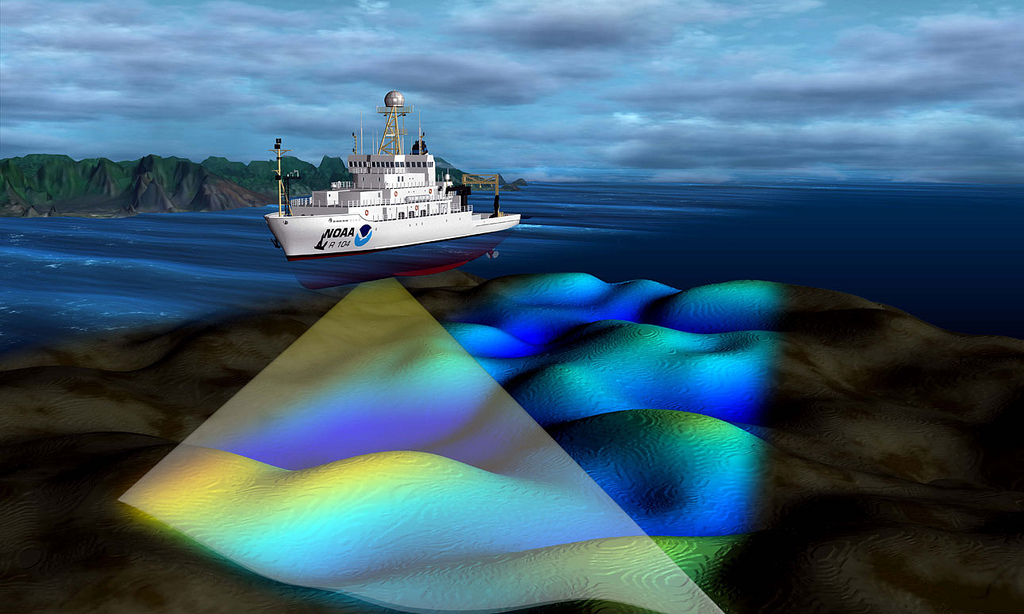
\includegraphics[width=.8\textwidth]{../Grade10/photos/sonar_NOAANationalOceanService_flickr.jpg}
% 
% \scalebox{0.8} % Change this value to rescale the drawing.
% {
% \begin{pspicture}(0,-3.93)(11.42,3.91)
% \definecolor{color78b}{rgb}{0.6,0.6,0.6}
% \psbezier[linewidth=0.04](0.52,-1.6283582)(3.3282945,-0.05)(4.980751,-1.0964925)(5.8,-2.11)(6.619249,-3.1235075)(8.99,-3.91)(10.64,-3.71)
% \psbezier[linewidth=0.04,fillstyle=solid,fillcolor=color78b](1.94,2.61)(1.9801459,1.77)(1.84,1.17)(2.44,1.15)(3.04,1.13)(6.68,1.01)(7.358321,1.29)(8.036642,1.57)(9.52,2.81)(8.58,2.59)(7.64,2.37)(1.96,2.43)(1.92,2.59)
% \psline[linewidth=0.04cm](2.52,2.49)(2.52,3.27)
% \psline[linewidth=0.04cm](2.52,3.27)(4.44,3.27)
% \psline[linewidth=0.04cm](4.44,3.27)(4.44,2.45)
% \psline[linewidth=0.04cm](3.14,3.81)(3.14,3.27)
% \psline[linewidth=0.04cm](3.76,3.81)(3.76,3.27)
% \psellipse[linewidth=0.04,dimen=outer](3.45,3.82)(0.33,0.09)
% \pscircle[linewidth=0.04,dimen=outer,fillstyle=solid,fillcolor=color78b](2.74,3.05){0.14}
% \pscircle[linewidth=0.04,dimen=outer,fillstyle=solid,fillcolor=color78b](3.18,3.05){0.14}
% \pscircle[linewidth=0.04,dimen=outer,fillstyle=solid,fillcolor=color78b](3.7,3.05){0.14}
% \pscircle[linewidth=0.04,dimen=outer,fillstyle=solid,fillcolor=color78b](4.12,3.05){0.14}
% \pscircle[linewidth=0.04,dimen=outer,fillstyle=solid,fillcolor=color78b](2.96,2.77){0.14}
% \pscircle[linewidth=0.04,dimen=outer,fillstyle=solid,fillcolor=color78b](3.44,2.77){0.14}
% \pscircle[linewidth=0.04,dimen=outer,fillstyle=solid,fillcolor=color78b](3.9,2.75){0.14}
% \rput(7.5798435,2.24){SAS Sonar}
% \psframe[linewidth=0.04,dimen=outer,fillstyle=solid](3.24,1.15)(3.02,1.05)
% \psframe[linewidth=0.04,dimen=outer,fillstyle=solid](4.58,1.13)(4.36,1.03)
% \pscustom[linewidth=0.04]
% {
% \newpath
% \moveto(9.94,1.31)
% }
% \psline[linewidth=0.04cm](0.0,1.61)(11.4,1.61)
% \psline[linewidth=0.04cm](3.12,1.15)(3.76,-0.85)
% \psline[linewidth=0.04cm](3.76,-0.85)(4.48,1.13)
% \psline[linewidth=0.04cm](3.2972062,0.25496995)(3.4476187,0.11434252)
% \psline[linewidth=0.04cm](3.4476187,0.11434252)(3.4875562,0.316345)
% \psline[linewidth=0.04cm](4.229458,0.10226333)(4.187863,0.30393106)
% \psline[linewidth=0.04cm](4.187863,0.30393106)(4.0386105,0.1620733)
% \rput(3.2217188,-1.2){seabed}
% \rput(1.949375,0.62){transmitter}
% \rput(5.47,0.62){receiver}
% \psline[linewidth=0.04cm,arrowsize=0.05291667cm 2.0,arrowlength=1.4,arrowinset=0.4]{->}(2.56,0.81)(3.0,1.03)
% \psline[linewidth=0.04cm,arrowsize=0.05291667cm 2.0,arrowlength=1.4,arrowinset=0.4]{->}(4.92,0.79)(4.64,1.03)
% %\psline[linewidth=0.04cm,arrowsize=0.05291667cm %2.0,arrowlength=1.4,arrowinset=0.4]{->}(6.36,-0.09)(6.36,-0.09)
% \rput(7.020781,-0.46){sea}
% \end{pspicture}
% }
\end{center}
\end{figure}       
\end{minipage}
\begin{minipage}{.5\textwidth}
Skepe maak gebruik van die weerkaatsingseienskappe van klankgolwe om die diepte van die oseaan te bereken. 'n Klankgolf word oorgedra en weerkaats van die seebodem af. Die spoed van klank in water is bekend en die tyd wat dit neem vir 'n klankgolf om terug te keer kan gemeet word. So kan die afstand na die bodem van die oseaan bereken word. Dit word sonar genoem, afkomstig van die Engels vir \textbf{So}und \textbf{N}avigation \textbf{A}nd \textbf{R}anging.\par    
 \end{minipage}
            

\begin{wex}{SONAR}{ 'n Skip stuur 'n sein na die bodem van die oseaan om die diepte te bereken. Die spoed van klank in water is is 1450 $\text{m}\cdot\text{s}^{-1}$ As die weerkaatse sein 1.5 sekondes later ontvang word, hoe diep is die oseaan by daardie punt?}{
\westep{Identifiseer wat gegee word en wat gevra word:}
\begin{eqnarray*}
s &=& 1450  \text{m.s^{-1}}\\
t &=& 1,5  \text{s}  \text{soontoe  en  terug}\\
\therefore t &= & 0,75 \text{s}  \text{een rigting}\\
d &=& ?
\end{eqnarray*}

\westep{Bereken die afstand:}
\begin{eqnarray*}
\text{Afstand} &=& \text{spoed} \times \text{tyd} \\
d &=& s \times t \\
&=& 1450 m.s^{-1} \times 0,75 s \\
&=& 1087,5  \text{ m}
\end{eqnarray*}
}
\end{wex}
          
\subsection{Eggoplasing}
            \nopagebreak
        \label{m38800*id185251}Diere soos dolfyne en vlermuise maak gebuik van klankgolwe om hulle pad te vind. Net soos skepe, gebruik vlermuise ook sonar om afstande na voorwerpe te bereken en sodoende hindernisse te vermy. Klankgolwe word uitgestuur en weerkaats van voorwerpe af rondom die vlermuis. Vlermuise en dolfyne maak gebruik van die weerkaatse klanke om 'n prentjie te vorm van wat om hulle is. Dit word eggoplasing genoem.\par



\section{Eienskappe van 'n klankgolf}
            \nopagebreak
      \label{m38799*id183478}Aangesien klank 'n golf is, kan ons die eienskappe van klank in verband bring met di\'{e} golwe. Die basiese eienskappe van klank is toonhoogte en hardheid.\par 

    \begin{figure}[h!tbp]
\begin{center}
%\scalebox{0.8}
%{
\begin{pspicture}(-5,-1)(5,1)%\psgrid
\psplot[xunit=0.0055,]{-360}{360}{x sin }
\psline[linestyle=dashed](-2,0)(2.5,0)
\psline[linestyle=dashed](-2,1)(2.5,1)
\psline[linestyle=dashed](-2,-1)(2.5,-1)
\psline{<->}(-2,-1.2)(-2,1.2)
\rput(-3.5,0){Klank A}
\end{pspicture}
%}
\end{center}

\begin{center}
%\scalebox{0.8}
%{
\begin{pspicture}(-5,-1)(5,2)%\psgrid
\psplot[xunit=0.0055,]{-360}{360}{-1 0.5 x mul sin mul}
\psline[linestyle=dashed](-2,0)(2.5,0)
\psline[linestyle=dashed](-2,1)(2.5,1)
\psline[linestyle=dashed](-2,-1)(2.5,-1)
\psline{<->}(-2,-1.2)(-2,1.2)
\rput(-3.5,0){Klank B}
\end{pspicture}
%}
\end{center}

\begin{center}
%\begin{minipage}{0.3\textwidth}
%\scalebox{0.8}
%{
\begin{pspicture}(-5,-1)(5,2)%\psgrid
\psplot[xunit=0.0055,]{-360}{360}{-1.5 0.5 x mul sin mul}
\psline[linestyle=dashed](-2,0)(2.5,0)
\psline[linestyle=dashed](-2,1)(2.5,1)
\psline[linestyle=dashed](-2,-1)(2.5,-1)
\psline{<->}(-2,-1.2)(-2,1.2)
\rput(-3.5,0){Klank C}
\end{pspicture}
%}
%\end{minipage}
\end{center}
\caption{Toonhoogte en hardheid van klank. Klank B het 'n \emph{laer} toonhoogte (laer frekwensie) as klank A en is \emph{sagter} (kleiner amplitude) as klank C.}\label{fig:pitchetc}
\end{figure}
      \label{m38799*uid2}
            \subsubsection{Toonhoogte}
            \nopagebreak
            
Die frekwensie van 'n klankgold is wat jy hoor as toonhoogte. 'n Ho\"er frekwensie klank het 'n ho\"er toonhoogte en 'n laer frekwensie klank het 'n laer toonhoogte. In Figuur~\ref{fig:pitchetc} het Klank A 'n ho\"er toonhoogte as Klank B. 'n Vo\"eltjie se sang sal byvoorbeeld 'n laer toonhoogte h\^e as die brul van 'n leeu.\par

Die menslike oor kan 'n wye verskeidenheid frekwensies hoor. Frekwensies van 20 tot 20 000 Hz is hoorbaar vir mense. Enige klank met 'n frekwensie onder 20 Hz word genoem \textbf{infraklank} en 'n klank met 'n frekwensie bo 20 000 Hz word genoem \textvf{ultraklank}.\par


Tabel~\ref{p:wsl:s11:rangeoff} lys die frekwensiebereik van sommige algemene diere rin vergeleke met mense.

\begin{table}[htbp]
\begin{center}
\caption{Omvang van frekwensie}
\label{p:wsl:s11:rangeoff}
\begin{tabular}{|l|c|c|}\hline
&onderste frekwensie (Hz) & boonste frekwensie (Hz)\\\hline\hline
Mense & 20 & 20 000\\\hline
Honde & 50 & 45 000\\\hline
Katte & 45 & 85 000\\\hline
Vlermuise & 20 & 120 000\\\hline
Dolfyne & 0,25 & 200 000\\\hline
Olifante & 5 & 10 000\\\hline
\hline
\end{tabular}
\end{center}
\end{table}
    \par
\begin{activity}{Reikwy\'ate van golflengte}
\nopagebreak
Gebruik die inligting in Tabel \ref{p:wsl:s11:rangeoff} om die laagste en hoogste golflengtes wat elke spesie kan hoor te bereken. Aanvaar dat die spoed van klank in lug 344 $m \cdot s^{-1}$ is.
\end{activity}
 
\subsubsection{Hardheid}
\nopagebreak

Die amplitude van 'n klankgolf beheer sy hardheid of volume. 'n Groter amplitude  beteken 'n harder klank en 'n kleiner amplitude beteken 'n sagter klank. In Figuur~\ref{fig:pitchetc} is Klank C harder as Klank B. Die vibrasie van 'n bron bepaal die amplitude van die golf. Energie word in die medium voortgeplant deur vibrasie. Meer energiele vibrasie stem ooreen met 'n groter amplitude want die deeltjies beweeg heftiger heen en weer. \par

Die hardheid van 'n klank word ook bepaal deur die sensitiwiteit van die oor. Die menslike oor is meer sensitief vir sekere frekwensies as ander. Die volume wat ons hoor is dus afhanklik van beide die amplitude van 'n klank asook die frekwensie van die klank.\par


\begin{exercises}{Klank, frekwensie en amplitude}
\nopagebreak
Bestudeer die volgende diagram wat 'n musieknoot voorstel
Skets die diagram vir 'n noot wat
\begin{enumerate}[noitemsep, label=\textbf{\arabic*}. ] 
\item 'n ho\"er toonhoogte het
\item harder is
\item sagter is
\end{enumerate}



\begin{figure}[H] % horizontal\label{m38799*id184017}
    \begin{center}
    \begin{pspicture}(-3,-1)(5,1)%\psgrid
\psplot[xunit=0.0055,]{-360}{360}{x sin }
\psline[linestyle=dashed](-2,0)(2.5,0)
\psline[linestyle=dashed](-2,1)(2.5,1)
\psline[linestyle=dashed](-2,-1)(2.5,-1)
\psline{<->}(-2,-1.2)(-2,1.2)
\end{pspicture}
    \end{center}
 \end{figure}               
 \par 
  \label{m38799**end}
\practiceinfo
 \par \begin{tabular}[h]{cccccc}
 (1.) 02ce  & \end{tabular}

\end{exercises}

\begin{activity}{Vergelyk instrumente wat klank genereer}
Die grootte en vorm van instrument be\"invloed die klanke wat hulle produseer. Kry 'n paar instrumente wat verskillende fisiese eienskappe het en vergelyk hulle klanke vergelyk. Jy kan:\par\vspace{1em}
\begin{minipage}{.45\columnwidth}
\textbf{Opsie 1: Vuvuzelas}\\
Die klank van vuvuzelas van verskillende groottes deur hulle te blaas.
Jy sal 'n paar verskillende vuvuzelas moet opspoor. Maak beurte om deur hulle te blaas, een op 'n slag en maak 'n nota van watter een jy dink is harder (amplitude) en watter een het 'n ho\"er toonhoogte (frekwensie).
\end{minipage}\hspace{.05\columnwidth}
\begin{minipage}{.45\columnwidth}
\textbf{Opsie 2: Stemvurke}\\
Vergelyk die klanke wat jy hoor as jy verskillende stemvurke tik.
Jy sal 'n paar verskillende stemvurke benodig. Maak beurte om hulle te tik, een op 'n slag en maak 'n nota van watter jy dink is harder (amplitude) en watter het ho\"er toonhoogte (frekwensie).
\end{minipage}\\
\textbf{Opsie 3: Seinopwekker en ossilloskoop}\\
Gebruik 'n seinopwekker om klanke met verskillende frekwensies en amplitudes te genereer en gebruik 'n ossilloskoop om die verskillende seine te bestudeer.\\
\begin{minipage}{.5\textwidth}
\textbf{Sein generator}\\
Die sein generator laat jou toe om die hardheid en frekwensie van die klank wat deur die luispreker gespeel word te beheer. Dit het kontroles vir amplitude en frekwensie.\\
\end{minipage}
\begin{minipage}{.5\textwidth}
\begin{center}
\textbf{ 'n Sein generator}\\
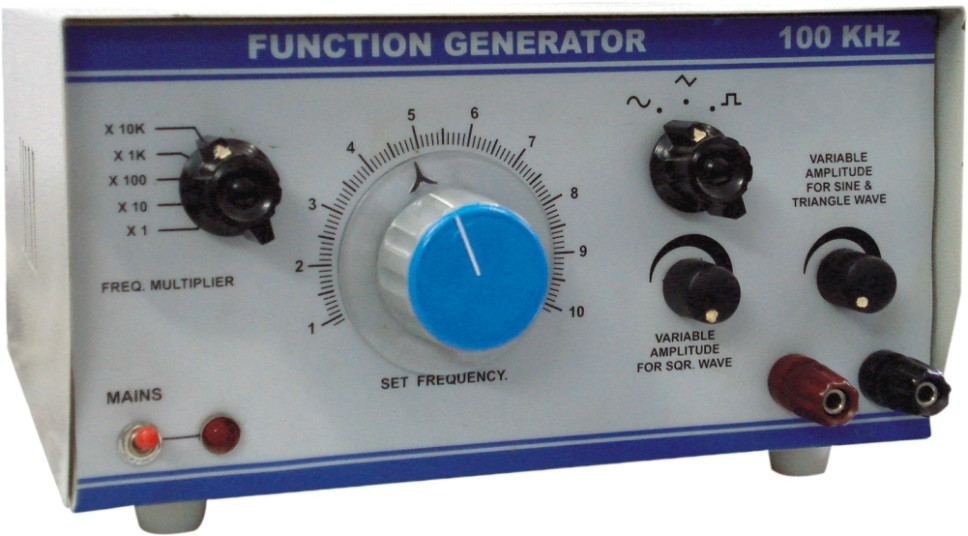
\includegraphics[width=.8\textwidth]{../Grade10/photos/function_generator.jpg}\\
\textsl{Foto deur Audin op Flickr}\\
\end{center}
\end{minipage}

\begin{minipage}{.5\textwidth}

\textbf{Osilloskoop} \\
Die mikrofoon kan dan die klank optel en dit omskakel na 'n elektriese sein wat op die ossiloskoop gesien kan word.\\

Die mees algemene ossiloskope het kontroles vir amplitude, frekwensie, snellers en kanale. Sodra jou onderwyser jou gehelp het om 'n sein op te spoor met die korrekte kanaal en sneller, kan jy die amplitude en frekwensie kontroles gebruik om die klank te bestudeer.\\

Die amplitude kontrole van 'n ossiloskoop beheer hoe hoog 'n gegewe potentiaal op die skerm vertoon. Die doel hiervan is sodat jy 'n groot en klein sein gelyktydig op die skerm kan vertoon. \\

\end{minipage}
\begin{minipage}{.5\textwidth}
\begin{center}
\textbf{An oscilloscope}\\
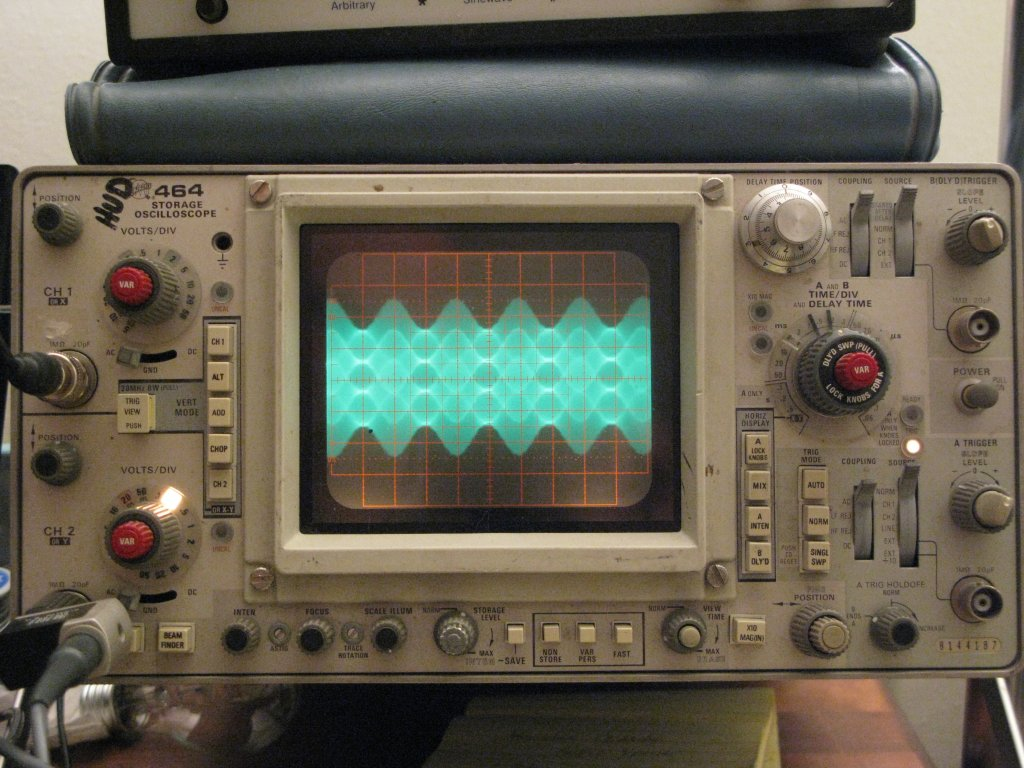
\includegraphics[width=.8\textwidth]{../Grade10/photos/oscilloscope_Audin_Flickr.jpg}\\
\textsl{Photograph by Audin on Flickr}\\
\textbf{Two different oscilloscope traces}\\
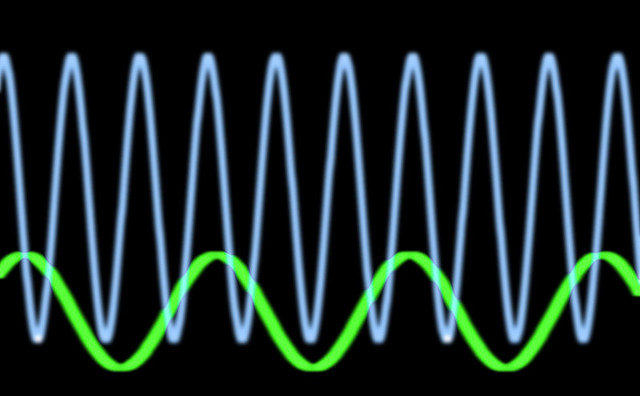
\includegraphics[width=.8\textwidth]{../Grade10/photos/oscilloscopetrace_Creativity103_Flickr.jpg}\\
\textsl{Photograph by Audin on Flickr}\\
\end{center}
\end{minipage}

\begin{minipage}{.5\textwidth}
 	
Die frekwensie (of tyd) kontrole van 'n ossiloskoop is hoeveel tyd 'n sekere afstand op die skerm verteenwoordig. Die doel hiervan is om 'n sein wat vinnig verander en een wat stadig verander gelyktydig op die skerm te kan vertoon.\\
\end{minipage}
\begin{minipage}{.5\textwidth}
\begin{center}
\begin{minipage}{.8\textwidth}
\vspace{.5cm}\textsl{\textbf{Nota:} Die beeld op die ossilloskoop sal vir jou 'n transversale gold patroon wys. Dit beteken nie dat klankgolwe transversaal is nie, dit wys dat die druk wat gemeet word wissel om dat klank 'n drukgolf is.}
\end{minipage}
\end{center}
\end{minipage}
\vspace{1em}\\
Jy sal met verskillende amplitudes en frekwensies kan eksperimenteer met die sein generator en sien wat gebeur met die golfvorm wat deru die mikrofoon opgetel word.\\


\end{activity}

%\Note{The display of the oscilloscope will show you a transverse wave pattern. This does not mean that klank waves are transverse waves but just shows that the pressure being measured is fluctuating because of a pressure wave.}

\mindsetvid{Veritasium Ruben's tube}{VPebn}

\section*{Intensiteit van klank}
\nopagebreak

\par
Intensiteit is een aanwyser van amplitude. Intensiteit is die energie wat deur 'n eenheid oppervlakte elke sekonde uitgestraal word.\par

Die eenheid van intensiteit is die \textbf{desibel} (simbool: dB).

\begin{table}[H]
\begin{center}
\begin{tabular}{|l|c|c|}\hline
\textbf{Bron}&\textbf{Intensiteit} (dB) & \textbf{Keer groter as gehoordrumpel}\\\hline
Vuurpyl lansering &180 & $10^{18}$\\
Straal vliegtuig & 140 & $10^{14}$ \\
Pyndrumpel & 120 & $10^{12}$\\
Rock orkes & 110 & $10^{11}$\\
%Subway Train & 90 & $10^{9}$\\
Fabriek & 80 & $10^{8}$\\
Stadsverkeer & 70 & $10^{7}$\\
Normale gesprek & 60 & $10^{6}$\\
Biblioteek & 40 & $10^{4}$\\
Fluister & 20 & $10^{2}$\\
Gehoordrumpel & 0 & 0\\
\hline
\end{tabular}
\end{center}
\caption{Voorbeelde van klank intensiteite.}
\label{p:wsl:s11:intensity}
\end{table}

Vuvuzelas is prominent by sokker wedstryde in Suid-Afrika. Die intensiteit van die klank van 'n vuvuzela is afhanklik van die afstand na die vuvuzela toe. In Tabel~\ref{table:vuvuzelas} kan jy sien hoe die intensiteit verskil

\begin{minipage}{.5\textwidth}
\begin{table}[H]
\begin{tabular}{ccccc}\hline
Frekwensie (Hz) & In oor & Oorskulp & 1 m & 2 m \\ \hline
125&   36  	&62	 &38	& 35 \\ \hline
250&	92 &	106	& 82	&	 85 \\ \hline
500&	103 & 121&	 102&	 101 		\\ \hline
1 000&	106 & 122&	 108&	 100 	\\  \hline
2 000&	101 & 122&	 110&	 101 	\\ \hline
4 000&	97 & 109&	 110&	 102 	\\ \hline
5 000&	93 & 111&	 109&	 100 		\\ \hline
8 000&  87 & 110&	 107&		 98 	\\ \hline
\end{tabular}
\label{table:vuvuzelas}
\caption{Gemiddelde vuvuzela intensiteit metings by verskillende frekwensies by 4 afsonderlike af-stande van die opening van die vuvuzela af (dBA). Tabel geneem uit South African Medical Journal (Cape Town, South Africa) \textbf{100} (4): 192}
\end{table}
\end{minipage}
\begin{minipage}{.5\textwidth}
\begin{center}
\textbf{Vuvuzelas in aksie}\par
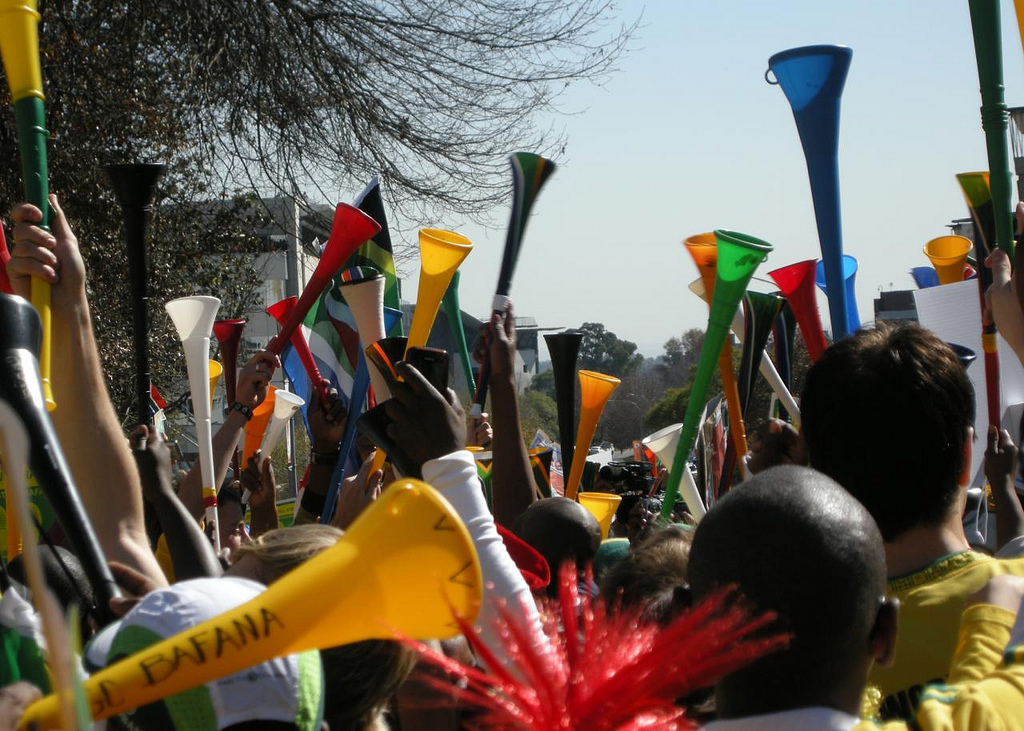
\includegraphics[width=.8\columnwidth]{../Grade10/photos/vuvuzelas_dundas_football_club.jpg}\par
Foto deur Dundas Football Club op Flickr.	
\end{center}
\end{minipage}

            
\section{Ultraklank}
            \nopagebreak
Ultraklank is klank met 'n frekwensie meer as 20 kHz. Sommige diere, soos honde, dolfyne en vlermuise, se gehoorbereik is ho\"er as di\'e van mense en kan ultraklank hoor.
    % \textbf{m38800*eip-558}\par
          \begin{table}[H]
    % \begin{table}[H]
    % \\ '' '0'
        \begin{center}
      \label{m38800*eip-558}
    \noindent
    \tabletail{%
        \hline
        \multicolumn{3}{|p{\mytableboxwidth}|}{\raggedleft \small \sl continued on next page}\\
        \hline
      }
      \tablelasttail{}
      \begin{xtabular}[t]{|l|c|c|}\hline
        Toepassing &
        Laagste frekwensie (kHz) &
        Hoogste frekwensie (kHz)% make-rowspan-placeholders
     \tabularnewline\cline{1-1}\cline{2-2}\cline{3-3}
      %--------------------------------------------------------------------
        Skoonmaak (bv. Juweliersware) &
        20 &
        40% make-rowspan-placeholders
     \tabularnewline\cline{1-1}\cline{2-2}\cline{3-3}
      %--------------------------------------------------------------------
        Toets vir foute in materiale &
        50 &
        500% make-rowspan-placeholders
     \tabularnewline\cline{1-1}\cline{2-2}\cline{3-3}
      %--------------------------------------------------------------------
        Sweis van plastiek &
        15 &
        40% make-rowspan-placeholders
     \tabularnewline\cline{1-1}\cline{2-2}\cline{3-3}
      %--------------------------------------------------------------------
     Gewas wegsnyding &
        250 &
        2000% make-rowspan-placeholders
     \tabularnewline\cline{1-1}\cline{2-2}\cline{3-3}
      %--------------------------------------------------------------------
    \end{xtabular}
      \end{center}
    \caption{Verskillende gebruike van ultraklank en die toepaslike frekwensies.}
\end{table}
    \par
  \par 

\begin{minipage}{.5\textwidth}
\begin{center}
\textbf{Ultraklank beeld van 'n ongebore baba}\par
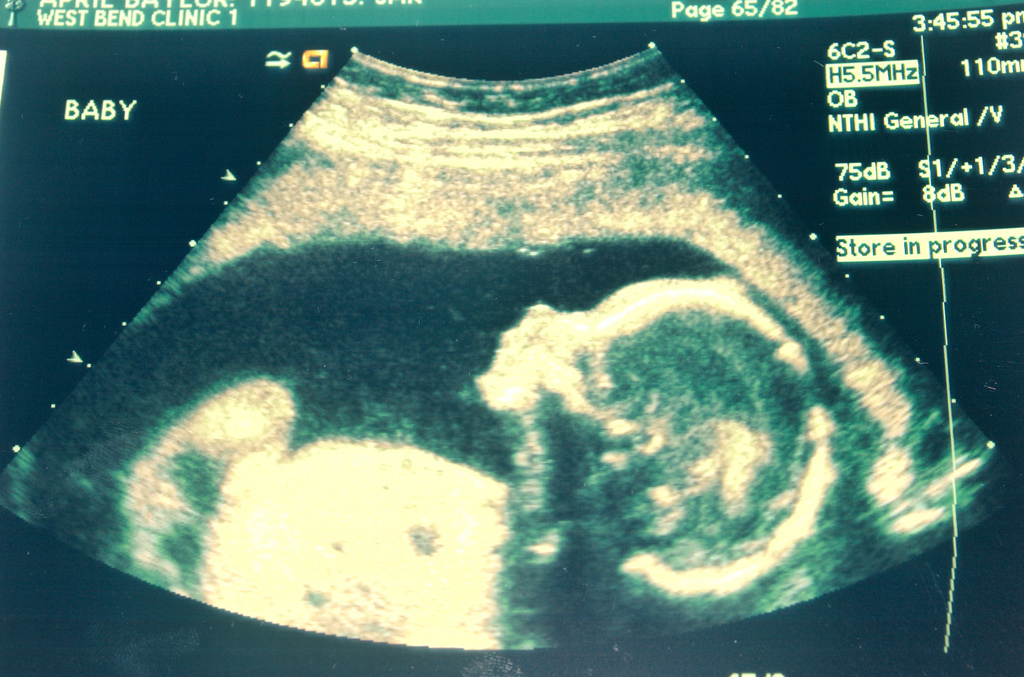
\includegraphics[width=.8\columnwidth]{../Grade10/photos/ultrasound_mbaylor_flickr.jpg}
\par\textit{Beeld deur mbaylor op Flickr.}
\end{center}
\end{minipage}
\begin{minipage}{.5\textwidth}

Die mees algemene gebruik van ultraklank is beeldskepping in industri\"ele en mediese toepassings. Die gebruik van ultraklank om beelde te skep is gebaseer op die weerkaatsing en oordrag van 'n golf by 'n grens (wanneer die golf van een materiaal na 'n ander beweeg). Wanneer 'n ultraklankgolf binne-in 'n voorwerp wat van verskillende materiale gemaak is beweeg, word die golf gedeeltelik weerkaats en oorgedra as dit by 'n grens kom, bv. tussen been en spier of spier en vet. Die deel van die golf wat weerkaats is kan dan opgeneem word en gebruik word om 'n beeld van die voorwerp te vorm. \par

Ultraklank in die medisyne word gebruik om spier en sagte weefsel te visualiseer, wat dit handig maak om na organe te kyk, en word ook gereeld gebruik tydens swangerskappe. Ultraklank is 'n veilige, nie-indringende metode om binne die menslike liggaam te kyk. \par
      
\end{minipage}

Bronne van ultraklank kan gebruik word om gelokaliseerde areas in biologiese weefsel te verhit, met toepassing in fisioterapie en kanker behandeling. Gefokusde ultraklank bronne word ook gebruik om nierstene op te breek.\par

Ultrasoniese skoonmakers, soms genoem supersoniese skoonmakers, word by frekwensies van 20-40kHz gebruik om juweliersware, lense en ander optiese dele, horlosies, tandheelkundige instrumente, chirurgiese instrumente en ander industri\"ele onderdele skoon te maak.

Hierdie skoonmakers bestaan uit 'n houer met 'n vloeistof in die voorwerp wat skoongemaak word binne-in geplaas. Ultrasoniese golwe word dan in die vloeistof oorgedra. Die meganisme vir die skoonmaakaksie in 'n ultrasoniese skoonmaker is die energie wat vrygelaat word as daar miljoene mikroskopiese borrels wat in die vloeistof voorkom bars.\par
\label{m38800*notfhsst!!!underscore!!!id482}


\IFact{Ultraklank gen\-e\-ra\-tor\-/\-luid\-spre\-ker stelses word verkoop wat beweer hulle kan knaagdiere en insekte wegjaag, maar daar is geen wetenskaplike bewyse dat hierdie toestelle werk nie; beheerde toetse het bewys dat knaagdiere vinnig leer dat die stelsels skadeloos is.}

\section*{Fisika van die oor en die gehoor [Vir Kennis]}
            \nopagebreak
\begin{figure}[H]
\begin{center}
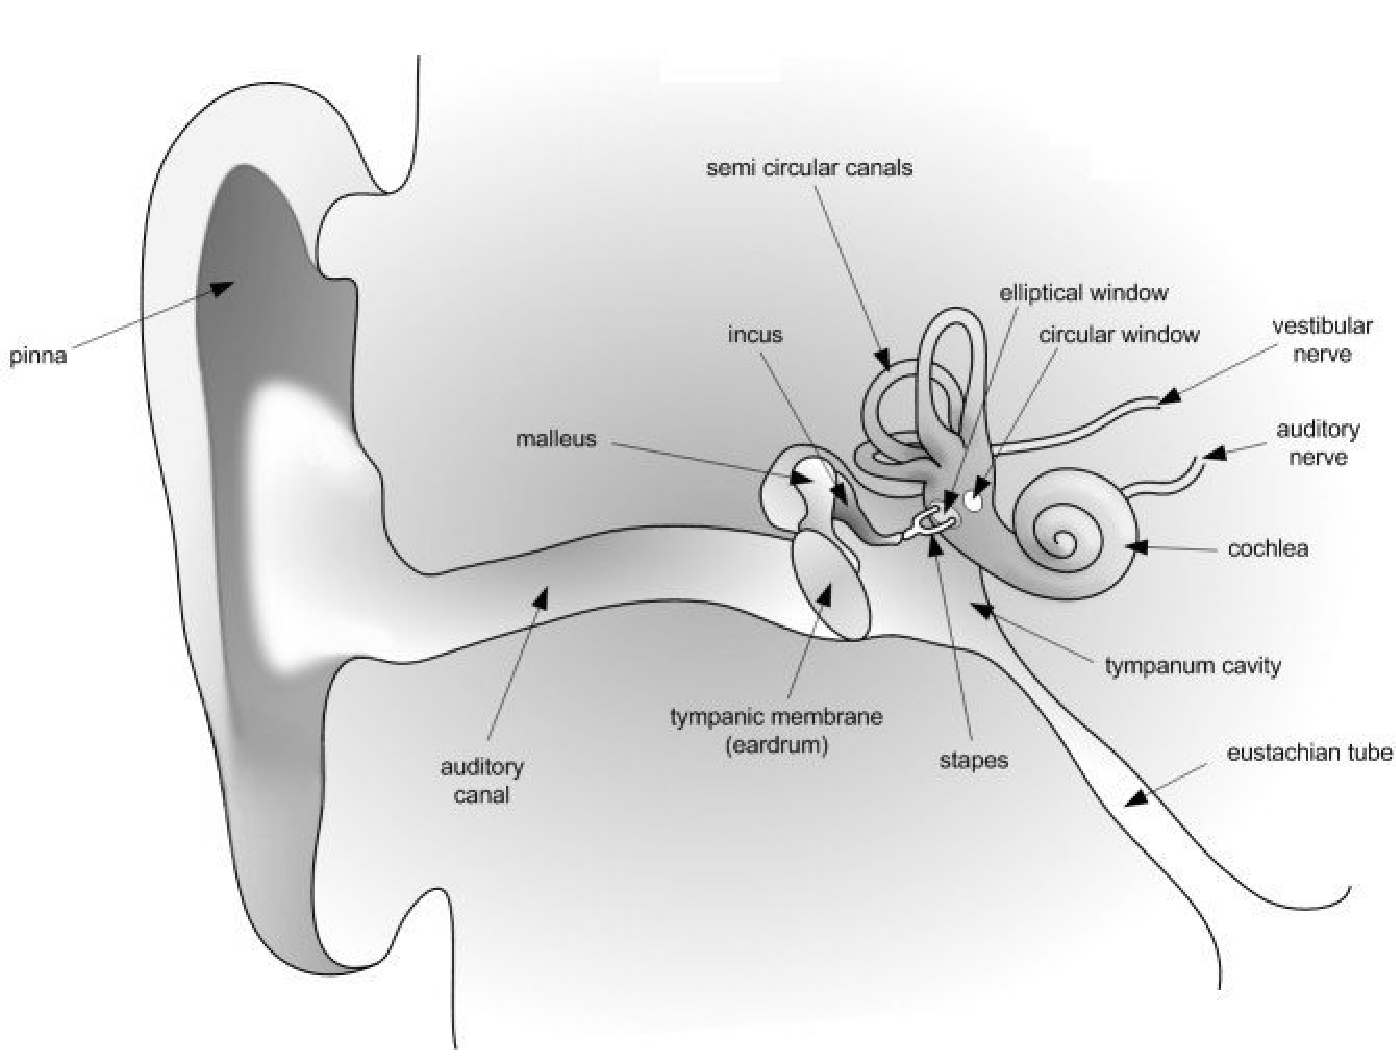
\includegraphics[width=0.65\textwidth]{HumanEar-GrayScale.pdf}
\end{center}
\caption{Diagram van die menslike oor }
\label{Human Ear}
\end{figure}


Die menslike oor is opgedeel in drie hoofdele: die buite-, middel- en binne-oor. Laat ons 'n klankgolf volg soos dit beweeg van die pinna (buitenste deel van oor) na die gehoor senuwee, wat 'n sein na die brein stuur. Die pinna is die deel van die oor waaraan ons tipies dink as ons van ore praat. Sy hoofdoel is om klankgolwe te vang en te fokus. Die golf beweeg dan deur die oorkanaal waarna dit die oordrom ontmoet. Die lugdrukvariasies van die klankgolf maak dat die oordrom vibreer. Die 3 klein beentjies van die middel-oor, die malleus (hamer), incus (aambeeldbeentjie) en stiebeuel dra dan die sein na die elliptiese venster toe. Dit is die begin van die binne-oor. Vandaar word die klank deur die vloeistof in die binne-oor versend en word as klank interpreteer deur die brein. Die binne-oor, wat van halfronde kanale gemaak is, die cochlea en die gehoorsenuwee is gevul met vloeistof. Die vloeistof laat die liggaam toe om vinnige bewegings te voel om balans te hou.
\par

Daar is klanke wat die pyndrumpel kan oorskry. Blootstelling aan hierdie klanke kan onmiddellike gehoorskade veroorsaak. In werklikheid kan blootstelling aan klanke oor 80 dB jou gehoor beskadig oor tyd. Stappe kan geneem word om skade te vermy, bv. deur oorpluisies of oormowwe aan te sit. Die beperking van voortdurende blootstelling asook die afstand tussen jou en die bron van die klank is ook belangrike stappe om te volg om jou gehoor te beskerm.\par

\pagebreak
\begin{groupdiscussion}{Belangrikheid van veiligheidstoerusting}
Werk in groepe van 5 en bespreek die belangrikheid van veiligheidstoerusting soos oorbeskerming, vir werkers in lawaaierige omgewings, bv. mense wat lugdrukbore gebruik of vliegtuie na hul parkeerareas aanwys. Skryf jou gevolg trekkings in 'n enkelbladsy verslag. 'n Bietjie navorsing mag miskien nodig wees om hierdie bespreking te voltooi.

\end{groupdiscussion} 
            \summary{VPecu}
            \nopagebreak
\begin{enumerate}[noitemsep, label=\textbf{\arabic*}. ] 
    \item Klankgolwe is longitudinaal
    \item Die \textbf{frekwensie} van 'n klank is 'n aanduiding van hoe hoog of hoe laag die \textsl{toonhoogte} van die klank is.
    \item Die menslike oor kan frekwensies tussen 20 tot 20~000 Hz hoor. \textbf{Infraklank} golwe het frekwensies onder 20 Hz. \textbf{Ultraklank} golwe het frekwensies bo 20~000 Hz.
    \item Die \textbf{amplitude} van 'n klank bepaal sy \textsl{hardheid} of volume.
    \item Die \textbf{toon} is 'n mate van die \textsl{kwaliteit} van 'n klank.
    \item Die spoed van klank in lug is omtrent $340\phantom{\rule{2pt}{0ex}}\text{m}\ensuremath{\cdot}\text{s}{}^{-1}$. Dit is afhanklik van die temperatuur, hoogte bo seevlak en die fase van die medium waardeur dit beweeg.
    \item Klank beweeg vinniger wanneer die medium warm is.
    \item Klank beweeg vinniger in 'n vaste stof as in 'n vloeistof en vinniger in 'n vloeistof as in 'n gas.
    \item Klank beweeg vinniger by seevlak waar die lugdruk ho\"er is.
    \item Die intensiteit van 'n klank is die energie wat deur 'n sekere area gedra word. Die intensiteit is 'n meting van frekwensie.
    \item Ultraklank kan gebruik word om beelde te vorm van dinge wat ons nie kan sien nie, bv. ongebore babas of gewasse.
    \item Eggoplasing word deur diere soos dolfyne en vlermuise gebruik om hulle omgewing te ``sien''.
    \item Skepe gebruik sonar om die diepte van die seebodem te meet of om skole visse op te spoor.
\end{enumerate}
            


\begin{eocexercises}{Klank}
            \nopagebreak
\begin{enumerate}[noitemsep, label=\textbf{\arabic*}. ] 
\item Kies \n woord van kolom B wat die konsep in kolom A die beste beskryf. 
    % \textbf{m38800*id185898}\par
          \begin{center}
\begin{tabular}{ll}
\textbf{Kolom A} & \textbf{Kolom B} \\ \hline
toonhoogte van klank \ \ \ & amplitude \\
hardheid van klank \ \ \ \ \ \ \ \ \ & frekwensie \\
kwaliteit van klank \ \ \ & spoed \\
& golfvorm \\
\end{tabular}
\end{center}
    \par
\item 'n Stemvurk, vioolsnaar en 'n luidspreker produseer klank. Dit is omdat hulle in 'n toestand van ...... is.
\begin{enumerate}[noitemsep, label=\textbf{\alph*}. ] 
    \item verdigting
    \item verdunning
    \item rotasie
    \item spanning
    \item vibrasie
\end{enumerate}

\item Wat sal 'n dromspeler doen om die klank wat die drom maak 'n laer toonhoogte te gee?
\begin{enumerate}[noitemsep, label=\textbf{\alph*}. ] 
    \item slaan die drom harder
    \item slaan die drom sagter
    \item slaan naby die rand van die drom
    \item maak die dromvel losser
    \item maak die dromvel stywer
\end{enumerate}

\item Wat is die ongeveerde frekwensiebereik van 'n gesonde mens?
\begin{enumerate}[noitemsep, label=\textbf{\alph*}. ] 
\item 0.2 Hz $\to $ 200 Hz
\item 2 Hz $\to $ 2 000 Hz
\item 20 Hz $\to $ 20 000 Hz
\item 200 Hz $\to $ 200 000 Hz
\item 2 000 Hz $\to $ 2 000 000 Hz
\end{enumerate}
                
\item X en Y is verskillende golwe. In lug beweeg X baie vinniger as Y maar het 'n baie korter golflengte. Watter tipe golwe kan X en Y wees? 
    % \textbf{m38800*id186268}\parIn l
          \begin{table}[H]
    % \begin{table}[H]
    % \\ 'id2920184' '1'
        \begin{center}
      \label{m38800*id186268}
    \noindent
          \tablelasttail{}
      \begin{xtabular}[t]{|l|l|l|}\hline
         &
        \uline{X} &
        \uline{Y}% make-rowspan-placeholders
     \tabularnewline\cline{1-1}\cline{2-2}\cline{3-3}
      %--------------------------------------------------------------------
        A &
        mikrogolwe &
        rooi lig% make-rowspan-placeholders
     \tabularnewline\cline{1-1}\cline{2-2}\cline{3-3}
      %--------------------------------------------------------------------
        B &
        radio &
        infrarooi% make-rowspan-placeholders
     \tabularnewline\cline{1-1}\cline{2-2}\cline{3-3}
      %--------------------------------------------------------------------
        C &
        rooi lig &
        klank% make-rowspan-placeholders
     \tabularnewline\cline{1-1}\cline{2-2}\cline{3-3}
      %--------------------------------------------------------------------
        D &
        klank &
        ultraviolet% make-rowspan-placeholders
     \tabularnewline\cline{1-1}\cline{2-2}\cline{3-3}
      %--------------------------------------------------------------------
        E &
        ultraviolet &
        radio% make-rowspan-placeholders
     \tabularnewline\cline{1-1}\cline{2-2}\cline{3-3}
      %--------------------------------------------------------------------
    \end{xtabular}
      \end{center}
\end{table}
    \par

\item Ruimtevaarders in 'n ruimteskip omwentel die maan. Hulle sien 'n ontploffing op die oppervlak van die maan. Hoekom kan hulle nie die ontploffing hoor nie?
\begin{enumerate}[noitemsep, label=\textbf{\alph*}. ] 
    \item Daar is nie ontploffings in die ruimte nie
    \item klank kan nie in 'n vakuum voortplant nie
    \item klank word weg vandie ruimteskip gereflekteer.
    \item klank beweeg te vinnig in die ruimte om die oor te be\"invloed.
    \item die ruimteskip beweeg teen 'n supersoniese spoed.
\end{enumerate}

\item 'n Man staan tussen twee kranse soos in die diagram hieronder, en klap sy hande een keer.
\begin{figure}[H] % horizontal\label{m38800*id186481}
\begin{center}
{
\begin{pspicture}(0,-1.0985937)(7.6665626,1.1185937)
\psline[linewidth=0.04cm](1.260625,0.92140627)(1.260625,-1.0785937)
\psline[linewidth=0.04cm](6.260625,0.94140625)(6.260625,-1.0585938)
%\usefont{T1}{ptm}{m}{n}
\rput(0.4575,0.47140625){krans 1}
%\usefont{T1}{ptm}{m}{n}
\rput(7.1339064,0.49140626){krans 2}
\psline[linewidth=0.04cm](1.260625,-1.0785937)(6.240625,-1.0585938)
\psline[linewidth=0.04cm](4.260625,0.88140625)(4.240625,0.52140623)
\psline[linewidth=0.04cm,arrowsize=0.1029cm 2.04,arrowlength=1.44,arrowinset=0.4]{<->}(1.240625,0.70140624)(4.240625,0.70140624)
\psline[linewidth=0.04cm,arrowsize=0.0929cm 2.05,arrowlength=1.45,arrowinset=0.4]{<->}(4.300625,0.70140624)(6.260625,0.70140624)
\pscircle[linewidth=0.04,dimen=outer](4.250625,0.21140625){0.25}
\psline[linewidth=0.04cm](4.240625,-0.05859375)(4.240625,-0.6585938)
\psline[linewidth=0.04cm](4.240625,-0.6585938)(3.940625,-1.0585938)
\psline[linewidth=0.04cm](4.240625,-0.6585938)(4.540625,-1.0585938)
\psline[linewidth=0.04cm](4.040625,-0.25859374)(4.440625,-0.25859374)
%\usefont{T1}{ptm}{m}{n}
\rput(2.6015625,0.94140625){\footnotesize 165 m}
%\usefont{T1}{ptm}{m}{n}
\rput(5.2015624,0.94140625){\footnotesize 110 m}
\end{pspicture}
}
\end{center}
 \end{figure}       
Maak die aanname dat die spoed van klank $330\phantom{\rule{2pt}{0ex}}m\ensuremath{\cdot}s{}^{-1}$ is. Wat sal die interval wees tussen die twee hardste eggos?
\begin{enumerate}[itemsep=5pt, label=\textbf{\alph*}. ] 
    \item $\dfrac{2}{3}\phantom{\rule{2pt}{0ex}}\text{s}$
    \item $\dfrac{1}{6}\phantom{\rule{2pt}{0ex}}\text{s}$
    \item $\dfrac{5}{6}\phantom{\rule{2pt}{0ex}}\text{s}$
    \item 1 s
    \item $\dfrac{1}{3}\phantom{\rule{2pt}{0ex}}\text{s}$
\end{enumerate}
\item 'n Dolfyn straal 'n ultrasoniese golf met 'n frekwensie van 0.15$MHz$ uit. Die spoed van die ultrasoniese golf is in water is 1500~m$\ensuremath{\cdot}$s${}^{-1}$. Wat is die golflengte van hierdie golf in water?
\begin{enumerate}[noitemsep, label=\textbf{\alph*}. ] 
    \item 0,1 mm
    \item 1 cm
    \item 10 cm
    \item 10 m
    \item 100 m
\end{enumerate}
                
\item Die amplitude en frekwensie van 'n klank word albei groter. Hoe word die hardheid en toonhoogte van die klank be\"invloed?
    % \textbf{m38800*id186726}\par
          \begin{table}[H]
    % \begin{table}[H]
    % \\ 'id2920575' '1'
        \begin{center}
      \label{m38800*id186726}
    \noindent
    \tabletail{%
        \hline
        \multicolumn{3}{|p{\mytableboxwidth}|}{\raggedleft \small \sl continued on next page}\\
        \hline
      }
      \tablelasttail{}
      \begin{xtabular}[t]{|l|l|l|}\hline
         &
        \uline{hardheid} &
        \uline{toonhoogte}% make-rowspan-placeholders
     \tabularnewline\cline{1-1}\cline{2-2}\cline{3-3}
      %--------------------------------------------------------------------
        A &
        vermeerder &
        verhoog% make-rowspan-placeholders
     \tabularnewline\cline{1-1}\cline{2-2}\cline{3-3}
      %--------------------------------------------------------------------
        B &
        vermeerder &
        onveranderd% make-rowspan-placeholders
     \tabularnewline\cline{1-1}\cline{2-2}\cline{3-3}
      %--------------------------------------------------------------------
        C &
        vermeerder &
        verlaag% make-rowspan-placeholders
     \tabularnewline\cline{1-1}\cline{2-2}\cline{3-3}
      %--------------------------------------------------------------------
        D &
        verminder &
        verhoog% make-rowspan-placeholders
     \tabularnewline\cline{1-1}\cline{2-2}\cline{3-3}
      %--------------------------------------------------------------------
        E &
        verminder &
        verlaag% make-rowspan-placeholders
     \tabularnewline\cline{1-1}\cline{2-2}\cline{3-3}
      %--------------------------------------------------------------------
    \end{xtabular}
      \end{center}
\end{table}
    \par

\item 'n Vegvliegtuig beweeg stadiger as die spoed van klank. Sy spoed is:
\begin{enumerate}[noitemsep, label=\textbf{\alph*}. ] 
\item Mach 1
\item supersonies
\item subsonies
\item hipersonies
\item infrasonies
\end{enumerate}
                
\item 'n Klankgolf is anders as 'n liggolf omdat 'n klankgolf:
\begin{enumerate}[noitemsep, label=\textbf{\alph*}. ] 
    \item deur 'n vibrerende voorwerp produseer word en lig nie.
    \item nie deur 'n vakuum kan trek nie.
    \item nie in staat is van diffraksie nie en lig is.
    \item in staat is om met 'n verskeidenheid frekwensies te bestaan en lig het net 'n enkele frekwensie. 
\end{enumerate}

\item By dieselfde temperatuur het klankgolwe die vinnigste spoed in:
\begin{enumerate}[noitemsep, label=\textbf{\alph*}. ] 
    \item klip
    \item melk
    \item suurstof
    \item sand
\end{enumerate}
                
\item Twee klankgolwe beweeg in 'n houer met stikstofgas. Die eerste golf het 'n golflengte van 1,5~m en die tweede golf het 'n golflengte van 4,5~m. Die spoed van die tweede golf is dus:
\begin{enumerate}[itemsep=5pt, label=\textbf{\alph*}. ] 
    \item $\dfrac{1}{9}$ die spoed van die eerste golf.
    \item $\dfrac{1}{3}$ die spoed van die eerste golf.
    \item dieselfde as die spoed van die eerste golf.
    \item drie keer meer as die spoed van die eerste golf.
    \item nege keer meer as die spoed van die eerste golf.
\end{enumerate}


\item Klank beweeg teen 'n spoed van 340~m$\ensuremath{\cdot}$s${}^{-1}$. 'n strooitjie is 0,25 m lank. Die staangolf wat in die strooitjie opgestel word met een kant toegemaak het 'n golflengte van 1,0~m. Die staangolf wat in die strooitjie opgstel is met albei kante toe se golflengte is 0,50 m.
\begin{enumerate}[noitemsep, label=\textbf{\alph*}. ] 
    \item Bereken die frekwensie van die klank wat jy kry as jy oor die strooitjie blaas met een kant toegemaak.
    \item Bereken die frekwensie van die klank wat jy kry as oor die strooitjie blaas met albei kante oop.
\end{enumerate}

\item 'n Donderstorm produseer weerlig and donderweer. Jy sien die weerlig amper onmiddelik omdat lig teen $3\ensuremath{\times}{10}^{8}\phantom{\rule{0.166667em}{0ex}}\text{m}\ensuremath{\cdot}{\text{s}}^{-1}$ beweeg. Nadat jy die weerlig gesien het, tel jy tot 5~s dan hoor jy die donderslag. Bereken die afstand na die storm toe.

\item 'n Persoon skreeu van die tweede verdieping van 'n huis na 'n ander persoon wat by die hek, 50 m weg, staan. as die sped van klank 344~m$\ensuremath{\cdot}$s${}^{-1}$ is, hoe lank vat dit die klank om die persoon wat by die hek staan te bereik?

\item  'n Stuk gereedskap het 'n waarskuwing op wat s\^e: "Waarskuwing! Hierdie instrument produseer 140 desibel". Watter voorsorgmaatre\"el behoort jy te neem voor jy die instrument aanskakel?

\item Watter eienskap van klank is 'n mate van die hoeveelheid energie wat die golf het?

\item Persoon 1 praat met Persoon 2. Verduidelik hoe die klank geproduseer word by Persoon 1 en hoe dit moontlik is vir Persoon 2 om die klank te hoor.

\item Klank kan nie voortplant in die ruimte nie. Bespreek watter ander metodes van kommunikasie ruimtevaarders kan gebruik as hulle buite hul ruimteskip is.

\item 'n Kamera met automatiese fokus gebruik 'n ultrasoniese klankgolf om op voorwerpe te fokus. Die kamera stuur klankgolwe uit wat van voorwerpe af weerkaats en dan terugkeer na die kamera. 'n Sensor meet die tyd wat dit vat vir die golwe om terug te keer en sodoende kan die afstand van die kamera af na 'n voorwerp gemeet word. As 'n klank golf (spoed = 344~m$\ensuremath{\cdot}$s${}^{-1}$) terugkeer na die kamera na 0,150~s, hoe ver weg is die voorwerp?

\item Bereken die frekwensie (in Hz) en golflengte van die irriterende klank wat 'n muskiet maak as dit sy vlerke teen 'n tempo van 600 keer per sekonde klap. Neem aan dat die spoed van klank golwe 344~m$\ensuremath{\cdot}$s${}^{-1}$ is.

\item Hoe be\"invloed die halvering van die frekwensie van 'n bron die spoed van die golwe wat geproduseer word?

\item Mense kan frekwensies hoor van tot 20~000 Hz. Neem aan dat die spoed van klank in lug 344~m$\ensuremath{\cdot}$s${}^{-1}$ is en bereken die golflengte van die klank wat ooreenstem met die boonste frekwensiebereik van menslike gehoor.

\item 'n Olifant trompetter teen 10~Hz. Neem aan dat die spoed van klank in lug 344~m$\ensuremath{\cdot}$s${}^{-1}$ is en bereken die golflengte van hierdie infrasoniese klank.

\item 'n Skip stuur 'n sein uit om die diepte van die oseaan te bepaal. Die sein keer terug na 2,5 sekondes. As die klank beweeg teen 1450~m$\ensuremath{\cdot}$s${}^{-1}$ in seewater, hoe diep is die oseaan op daardie punt?

\item 'n Persoon skreeu na 'n krans toe en hoor 'n eggo vanaf die krans 1~s later. As die spoed van klank 344~m$\ensuremath{\cdot}$s${}^{-1}$ is, hoe ver weg is die krans?

\item Kies 'n woord van Kolom B wat die beskrywing in Kolom die beste pas.
    % \textbf{m38783*id293899}\par
\begin{center}
\begin{tabular}{ll}
\textbf{Kolom A} & \textbf{Kolom B} \\ \hline
golwe in lug wat deur vibrasies veroorsaak is & longitudinale golwe \\
golwe wat in een rigting beweeg maar die medium beweeg in 'n ander & frekwensie \\
golwe en medium beweeg in dieselfde rigting  & geruis \\
die afstand tussen twee punte in 'n golf wat in fase is & amplitude \\
hoe gereeld 'n enkele golflengte verby beweeg & klankgolwe \\
die helfte van die afstand tussen die hoogste en laagste punte in 'n golf & staangolwe \\
die afstand wat 'n golf afl\^e in 'n tydsinterval & transversale golwe \\
die tyd wat dit vat vir een golflengte om verby 'n punt te beweeg & golflengte \\
& musiek \\
& klanke \\
& golfspoed \\
\end{tabular}
\end{center}
\end{enumerate}
  \label{m38800**end}
  \label{9b5d72dd5f0585e544578ab90a9956a8**end}
% Automatically inserted shortcodes - number to insert 28
\par \practiceinfo
\par \begin{tabular}[h]{cccccc}
% Question 1
(1.)	02cf	&
% Question 2
(2.)	02cg	&
% Question 3
(3.)	02ch	&
% Question 4
(4.)	02ci	&
% Question 5
(5.)	02cj	&
% Question 6
(6.)	02ck	\\ % End row of shortcodes
% Question 7
(7.)	02cm	&
% Question 8
(8.)	02cn	&
% Question 9
(9.)	02cp	&
% Question 10
(10.)	02cq	&
% Question 11
(11.)	02cr	&
% Question 12
(12.)	02cs	\\ % End row of shortcodes
% Question 13
(13.)	02ct	&
% Question 14
(14.)	02cu	&
% Question 15
(15.)	02cv	&
% Question 16
(16.)	02cw	&
% Question 17
(17.)	02cx	&
% Question 18
(18.)	02cy	\\ % End row of shortcodes
% Question 19
(19.)	02cz	&
% Question 20
(20.)	02d0	&
% Question 21
(21.)	02d1	&
% Question 22
(22.)	02d2	&
% Question 23
(23.)	02d3	&
% Question 24
(24.)	02d4	\\ % End row of shortcodes
% Question 25
(25.)	02d5	&
% Question 26
(26.)	02d6	&
% Question 27
(27.)	02d7	&
% Question 28
(28.)	02d8	&
\end{tabular}
% Automatically inserted shortcodes - number inserted 28
\end{eocexercises}
